\section{Versuchsaufbau und Methodik}
\label{chap:methodik}

Zur Charakterisierung der Messstromwandler wurde ein Hochstrom-Prüfstand eingesetzt, der primäre Wechselströme von bis zu \SI{6000}{A} generieren kann.
Dies ermöglicht die Analyse der magnetischen Eigenschaften sowie der Messgenauigkeit unter realitätsnahen Betriebsbedingungen.
Das methodische Vorgehen untergliedert sich in die technische Beschreibung der Basiskomponenten, die kritische Analyse des ursprünglichen Messkonzepts sowie die daraus resultierende Systemoptimierung für die finalen Messreihen.

\subsection{Hochstrom-Prüfstand}
\label{sec:hochstrom_pruefstand}

Der Hochstrom-Prüfstand dient der Erzeugung und Regelung hoher Wechselströme für thermische und elektrodynamische Untersuchungen an elektrischen Betriebsmitteln.
Als Prüflinge fungieren in der Regel Niederspannungsschaltanlagen oder deren Teilkomponenten, die unter Lastbedingungen auf ihre thermische Belastbarkeit geprüft werden.
Die Anlage ermöglicht die Bereitstellung von Strömen bis \SI{6000}{A} bei einer geringen Sekundärspannung.

\subsubsection{Aufbau und Funktionsweise}
\label{sec:aufbau_funktionsweise}

Der Leistungspfad beginnt primärseitig mit einem motorbetriebenen Säulenstelltransformator der Firma Ruhstrat, der mit einer Leistung von \SI{90}{kVA} als zentrales Stellglied fungiert.
Dem Transformator sind Netzdrosseln nachgeschaltet, die zur Entkopplung von Stromspitzen dienen.
Die Spannungsstellung erfolgt stufenlos über verstellbare Kohlerollbürsten, wodurch eine variable Ausgangsspannung zwischen \SI{0}{V} und \SI{380}{V} bereitgestellt wird.
Diese Spannung speist den nachgeschalteten Hochstrom-Festtransformator von Rolf Janssen (Typ UI 260/420 M).
Mit einer Nennleistung von \SI{30}{kVA} transformiert dieser die Spannung auf eine Kleinspannung von \SI{6}{V} herab, was sekundärseitig die Realisierung von Prüfströmen bis zu \SI{6000}{A} am dreiphasigen Abgang ermöglicht.

\begin{figure}[H]
    \centering
    \includegraphics[width=1.0\textwidth]{03_Ressourcen/zeichnungen/aufbau_hochstrom_pruefstand.drawio.pdf}
    \caption{Blockschaltbild des Hochstrom-Prüfstandes mit Leistungs- und Signalpfaden}
    \label{pic:aufbau_hochstrom_pruefstand}
\end{figure}

\subsubsection{Regelungskonzept}
\label{sec:regelungskonzept}

Die Stromregelung ist als digitaler \gls{pid}-Regelkreis innerhalb der Siemens \gls{et200s} realisiert.
Der Anwender gibt über die \gls{wincc}-Visualisierung den gewünschten Sollstrom vor, welchen die \gls{sps} kontinuierlich mit dem rückgeführten Istwert vergleicht.
Als Stellgröße generiert die Steuerung Schaltbefehle für den Antriebsmotor des Säulenstelltransformators.
Um permanentes Nachregeln zu minimieren, die starke Stromspitzen erzeugen, ist eine Hysterese als Totband in den Regelalgorithmus integriert.
Die Visualisierung übernimmt dabei neben der Parametrierung auch das lückenlose Datenlogging der Versuchsverläufe.
Eine detaillierte Spezifikation der einzelnen Komponenten ist in Tabelle~\ref{tab:komponenten_hochstrom} zusammengefasst.


\begin{table}[H]
    \centering
    \caption{Detaillierte Spezifikation der Komponenten}
    \label{tab:komponenten_hochstrom}
    \small
    % Definition:
    % X-Spalte am Ende für automatischen Umbruch bei langen Texten (wie 'Direct Current')
    \begin{tabularx}{\textwidth}{@{}l l l l >{\raggedright\arraybackslash}X@{}}
        \toprule
        \textbf{Komponente}      & \textbf{Typ}                  & \textbf{\makecell[l]{Leistung /                                                                                \\ Bürde}}
        
                                 & \textbf{\makecell[l]{Primär /                                                                                                                  \\ Input}} & \textbf{\makecell[l]{Sekundär /\\ Output}}                                                                                \\ \midrule
        Säulenstelltransformator & Ruhstrat                      & \SI{90}{kVA}

        
        
        
                                 & \SI{380}{V}                   & \SI{0}{V}--\SI{380}{V} (\SI{70}{A})                                                                            \\
        Festtransformator        & Janssen                       & \SI{30}{kVA}

        
        
        
                                 & \SI{380}{V}                   & \SI{6}{V} (\SI{5000}{A})                                                                                       \\
        Stromwandler             & Celsa ICG                     & \SI{5}{VA}

        
        
        
                                 & \SI{6000}{A}                  & \SI{5}{A} (Kl. 0,2S)                                                                                           \\
        
        Messumformer (K-3)       & 3-K Elektrik                  & --                                                                               & \SI{0}{A}--\SI{5}{A} AC & 
        \SI{0}{mA}--\SI{20}{mA} \gls{dc}                                                                                                                                          \\ \midrule
        \textbf{Leittechnik}     & \textbf{Typ}                  & \multicolumn{3}{l}{\textbf{Beschreibung}}

        
        
        
        \\ \cmidrule(r){1-2}
        % p{9cm} sorgt hier für den Umbruch in der verbundenen Zelle, damit die Tabelle nicht gesprengt wird
        Steuerung                & Siemens \gls{et200s}          & \multicolumn{3}{p{9cm}}{\gls{profinet}-Anbindung, Stromregelung, Analogeingänge}

        
        
        
        \\
        Visualisierung           & Siemens \gls{wincc}           & \multicolumn{3}{p{9cm}}{\gls{hmi}-System, Prozessüberwachung, Datenlogging}

        
        
        
        \\ \bottomrule
    \end{tabularx}
\end{table}


\subsubsection{Ursprünglicher Aufbau der Messstrecke}
\label{sec:aufbau_alter_messstrecke}

\begin{figure}[H]
    \centering
    \includegraphics[width=1.0\textwidth]{03_Ressourcen/zeichnungen/aufbau_messstrecke.drawio.pdf}
    \caption{Schematischer Aufbau der Messstrecke zur Ermittlung der Messabweichung}
    \label{pic:aufbau_messstrecke}
\end{figure}

Der erste Aufbau der Messstrecke (siehe Abbildung \ref{pic:aufbau_messstrecke}) sah zwei parallele Erfassungspfade vor.
Zur Bestimmung des Referenzwertes der Einspeisung wurden die K-3-Messumformer genutzt, welche das Signal an die \gls{sps} übermittelten.
Parallel dazu wurde das Ausgangssignal des Prüflings mit einem Digitalmultimeter von Fluke im Modus „Acquire“ erfasst.
%Die Inbetriebnahme diente dazu, die Funktionalität der Regelung sowie die Genauigkeit der Messwerterfassung unter Lastbedingungen zu verifizieren.

\subsubsection{Schwachstellen im Messkonzept}
\label{sec:fehleranalyse}

Die Auswertung der ersten Messreihen zeigt Abweichungen, die über den gesamten Messbereich auftreten.
In Abbildung \ref{pic:dia_messstrecke_alt} sind die Verläufe der Messumformer K-3 (blau) und der Rogowskispulen (orange) dargestellt.
Die Rogowskispulen wurden parallel eingesetzt, um deren Eignung für die Prüfung der Wandler zu untersuchen.
Beide Systeme erfassten die Messwerte zeitgleich an einem Messpunkt hinter dem Festtransformator.
Als Referenz dient die Genauigkeitsklasse 0,2, da die primärseitigen Stromwandler der Klasse 0,2S entsprechen.
Die grafische Darstellung verdeutlicht, dass beide Messsysteme die durch die Norm vorgegebenen Toleranzgrenzen (gestrichelte Linien) nicht einhalten.
In Phase L1 überschreitet der Messumformer K-3 ab einer Last von 50\,\% den positiven Grenzwert, während die Rogowskispulen eine negative Abweichung zwischen -1\,\% und -2,5\,\% aufweisen.
In Phase L2 zeigt der Messumformer K-3 bei 20\,\% Last einen Abfall der Genauigkeit auf circa -2\,\%, wohingegen die Rogowskispulen eine positive Abweichung von über 1\,\% erreichen.
Da die Verläufe der beiden Messsysteme voneinander abweichen, kann kein eindeutiger Referenzwert für den Primärstrom bestimmt werden.

\begin{diagram}[H]
    \centering
    \includegraphics[width=1.0\textwidth]{03_Ressourcen/diagramme/dia_messstrecke_alt/dia_messstrecke_alt-Zusammenfassung_MultiCurrent.pdf}
    \caption{Analyse der Messabweichung und Standardabweichung der Phasen L1, L2 und L3 im ursprünglichen Versuchsaufbau}
    \label{pic:dia_messstrecke_alt}
\end{diagram}


Die im unteren Teil der Abbildung \ref{pic:dia_messstrecke_alt} dargestellte Standardabweichung zeigt, dass beide Messgeräte im niedrigen Strombereich eine erhöhte Varianz aufweisen.
Dies ist darauf zurückzuführen, dass der Säulenstelltransformator bei geringen Strömen einen begrenzten Stellbereich besitzt, woraus eine geringere Stabilität des Stromwertes resultiert aus der Regelung.
Mit zunehmender Stromstärke reduziert sich dieses Rauschen im Messsignal. Dabei weisen die K-3-Messumformer eine geringere Schwankungsbreite auf als die Rogowskispulen.
Aufgrund dieser Ergebnisse sind beide Messverfahren für eine Referenzmessung im Rahmen der Genauigkeitsprüfung unzureichend.
Im folgenden Abschnitt \ref{sec:optimierung_messsystem} wird die Systemoptimierung erläutert, um eine präzisere Messwerterfassung zu realisieren.

\subsection{Optimiertes Messsystem}
\label{sec:optimierung_messsystem}

Wie im vorangegangenen Abschnitt dargelegt, erfüllte die ursprüngliche Messstrecke nicht die Anforderungen an eine präzise Genauigkeitsprüfung von Messstromwandlern.
Aus diesem Grund wurde eine Optimierung des Hochstrom-Prüfstandes durchgeführt. Das primäre Ziel dieser Maßnahmen war die Steigerung der Messgenauigkeit sowie die Automatisierung des Prüfablaufs, um reproduzierbare und direkt vergleichbare Ergebnisse sicherzustellen.
Zur technischen Umsetzung wurden zwei digitale Energiemessgeräte der Siemens-Produktfamilie ausgewählt.
Das Modell PAC3220, welches für die Erfassung des Prüflingsstroms eingesetzt wird \cite[S.~97]{siemens_pac3220_2019}, sowie das zur Überwachung der Einspeisung genutzte PAC4220 \cite[S.~94]{siemens_pac4220_2024} verfügen jeweils über die Genauigkeitsklasse 0,2 für die Strommessung.
Diese Geräte ermöglichen durch optionale Erweiterungsmodule eine direkte Integration in die Systemumgebung der Siemens \gls{et200s} via \gls{profinet}-Protokoll.
Ein wesentlicher Vorteil dieser Konfiguration liegt in der dezentralen Messwerterfassung unmittelbar am Messpunkt.
Dadurch lassen sich parasitäre Effekte über lange Messleitungen minimieren. Die Einbindung in die \gls{sps} erfolgt durch eine direkte zyklische Datenübertragung, wodurch die manuelle Abfrage von Registern entfällt und eine zeitsynchrone Datenbasis für beide Messpunkte geschaffen wird.

\begin{figure}[H]
    \centering
    \includegraphics[width=1.0\textwidth]{03_Ressourcen/zeichnungen/aufbau_hochstrom_pruefstand_new.drawio.pdf}
    \caption{Schematischer Aufbau der optimierten Messstrecke mit Siemens SENTRON Messgeräten}
    \label{pic:aufbau_messstrecke_neu}
\end{figure}

Die in Abbildung \ref{pic:aufbau_messstrecke_neu} dargestellte Systemarchitektur verdeutlicht die informationstechnische Vernetzung des optimierten Messaufbaus.
Während der obere Teil des Schemas den bereits beschriebenen Leistungspfad darstellt, erfolgt die messtechnische Erfassung der Primärströme zyklisch durch die Geräte PAC 4220 (Einspeisung) und PAC 3220 (Prüfling).
Die erfassten Stromwerte werden in \gls{wincc} archiviert und stehen dort für die Prozessüberwachung zur Verfügung.
Über die Benutzeroberfläche (\gls{hmi}) können diese Daten als \gls{csv}-Datei exportiert werden.
Diese Datei dient als Grundlage für die anschließende Genauigkeitsmessung und die Auswertung der Versuchsreihen.

\subsubsection{Systemintegration und Programmentwicklung}
\label{sec:integration_programmierung}

Die technische Umsetzung des optimierten Messsystems umfasst sowohl die informationstechnische Einbindung der Hardware-Komponenten als auch die Entwicklung der steuerungstechnischen Ablauflogik.
Zur Adressierung der SENTRON-Messgeräte wird jedem Gerät in der Hardware-Konfiguration des Simatic Managers ein eindeutiger Gerätename sowie eine IP-Adresse zugewiesen.
Diese Zuweisung ist notwendig, um die Kommunikation der Teilnehmer innerhalb des \gls{profinet}-Netzwerks mit der \gls{sps} zu ermöglichen.
Innerhalb des Hardware-Konfigurators werden die spezifischen Messwerte der Geräte auf die Eingangsadressen der \gls{sps} abgebildet.
Die so bereitgestellten Rohwerte werden im Anwenderprogramm der Steuerung aus dem Peripheriebereich ausgelesen und in \gls{db}s übertragen.
Der gesamte Quellcode der verwendeten Programmbausteine ist hierfür in Abschnitt \ref{chap:anhang_programm} aufgeführt.
Für die Erfassung der Daten in \gls{wincc} wird im Variablenhaushalt des Visualisierungssystems eine Kommunikationsverbindung zur Steuerung projektiert.
Die Variablen für die gemessenen Ströme werden direkt mit den entsprechenden Speicheradressen innerhalb der \gls{db}s verknüpft.
Über diese Verbindung werden die Werte der Ströme in regelmäßigen Abständen vom System ausgelesen, auf dem \gls{hmi} angezeigt und für den späteren Export als \gls{csv}-Datei in der Datenbank gespeichert.
Die Automatisierung des Prüfablaufs wird über die \gls{sps} realisiert, wobei der vorhandene \gls{pid}-Regler zur präzisen Stromeinstellung genutzt wird.
Für die Genauigkeitsmessung eines Wandlers sind gemäß Norm primär die Prüfpunkte bei 5~\%, 20~\%, 100~\% und 120~\% des Primär-Nennstroms von Bedeutung.
Um eine detailliertere Kennlinie zu erhalten und das Verhalten des Wandlers umfassender zu charakterisieren, wurden dem Prüfablauf weitere Messpunkte hinzugefügt.
Die automatisierte Erfassung umfasst somit die Pegel 5~\%, 20~\%, 50~\%, 80~\%, 90~\%, 100~\% und 120~\%.
Um diese Messpunkte automatisiert anzufahren, wurde eine Schrittkette entwickelt. Diese durchläuft die Prüfpegel sequenziell und hält jeden Messpunkt für eine Dauer von fünf Minuten konstant.
Dieser Zeitraum gewährleistet eine ausreichende thermische Sättigung des Wandlerkerns und ermöglicht eine valide Mittelwertbildung der Messdaten.

\begin{figure}[H]
    \centering
    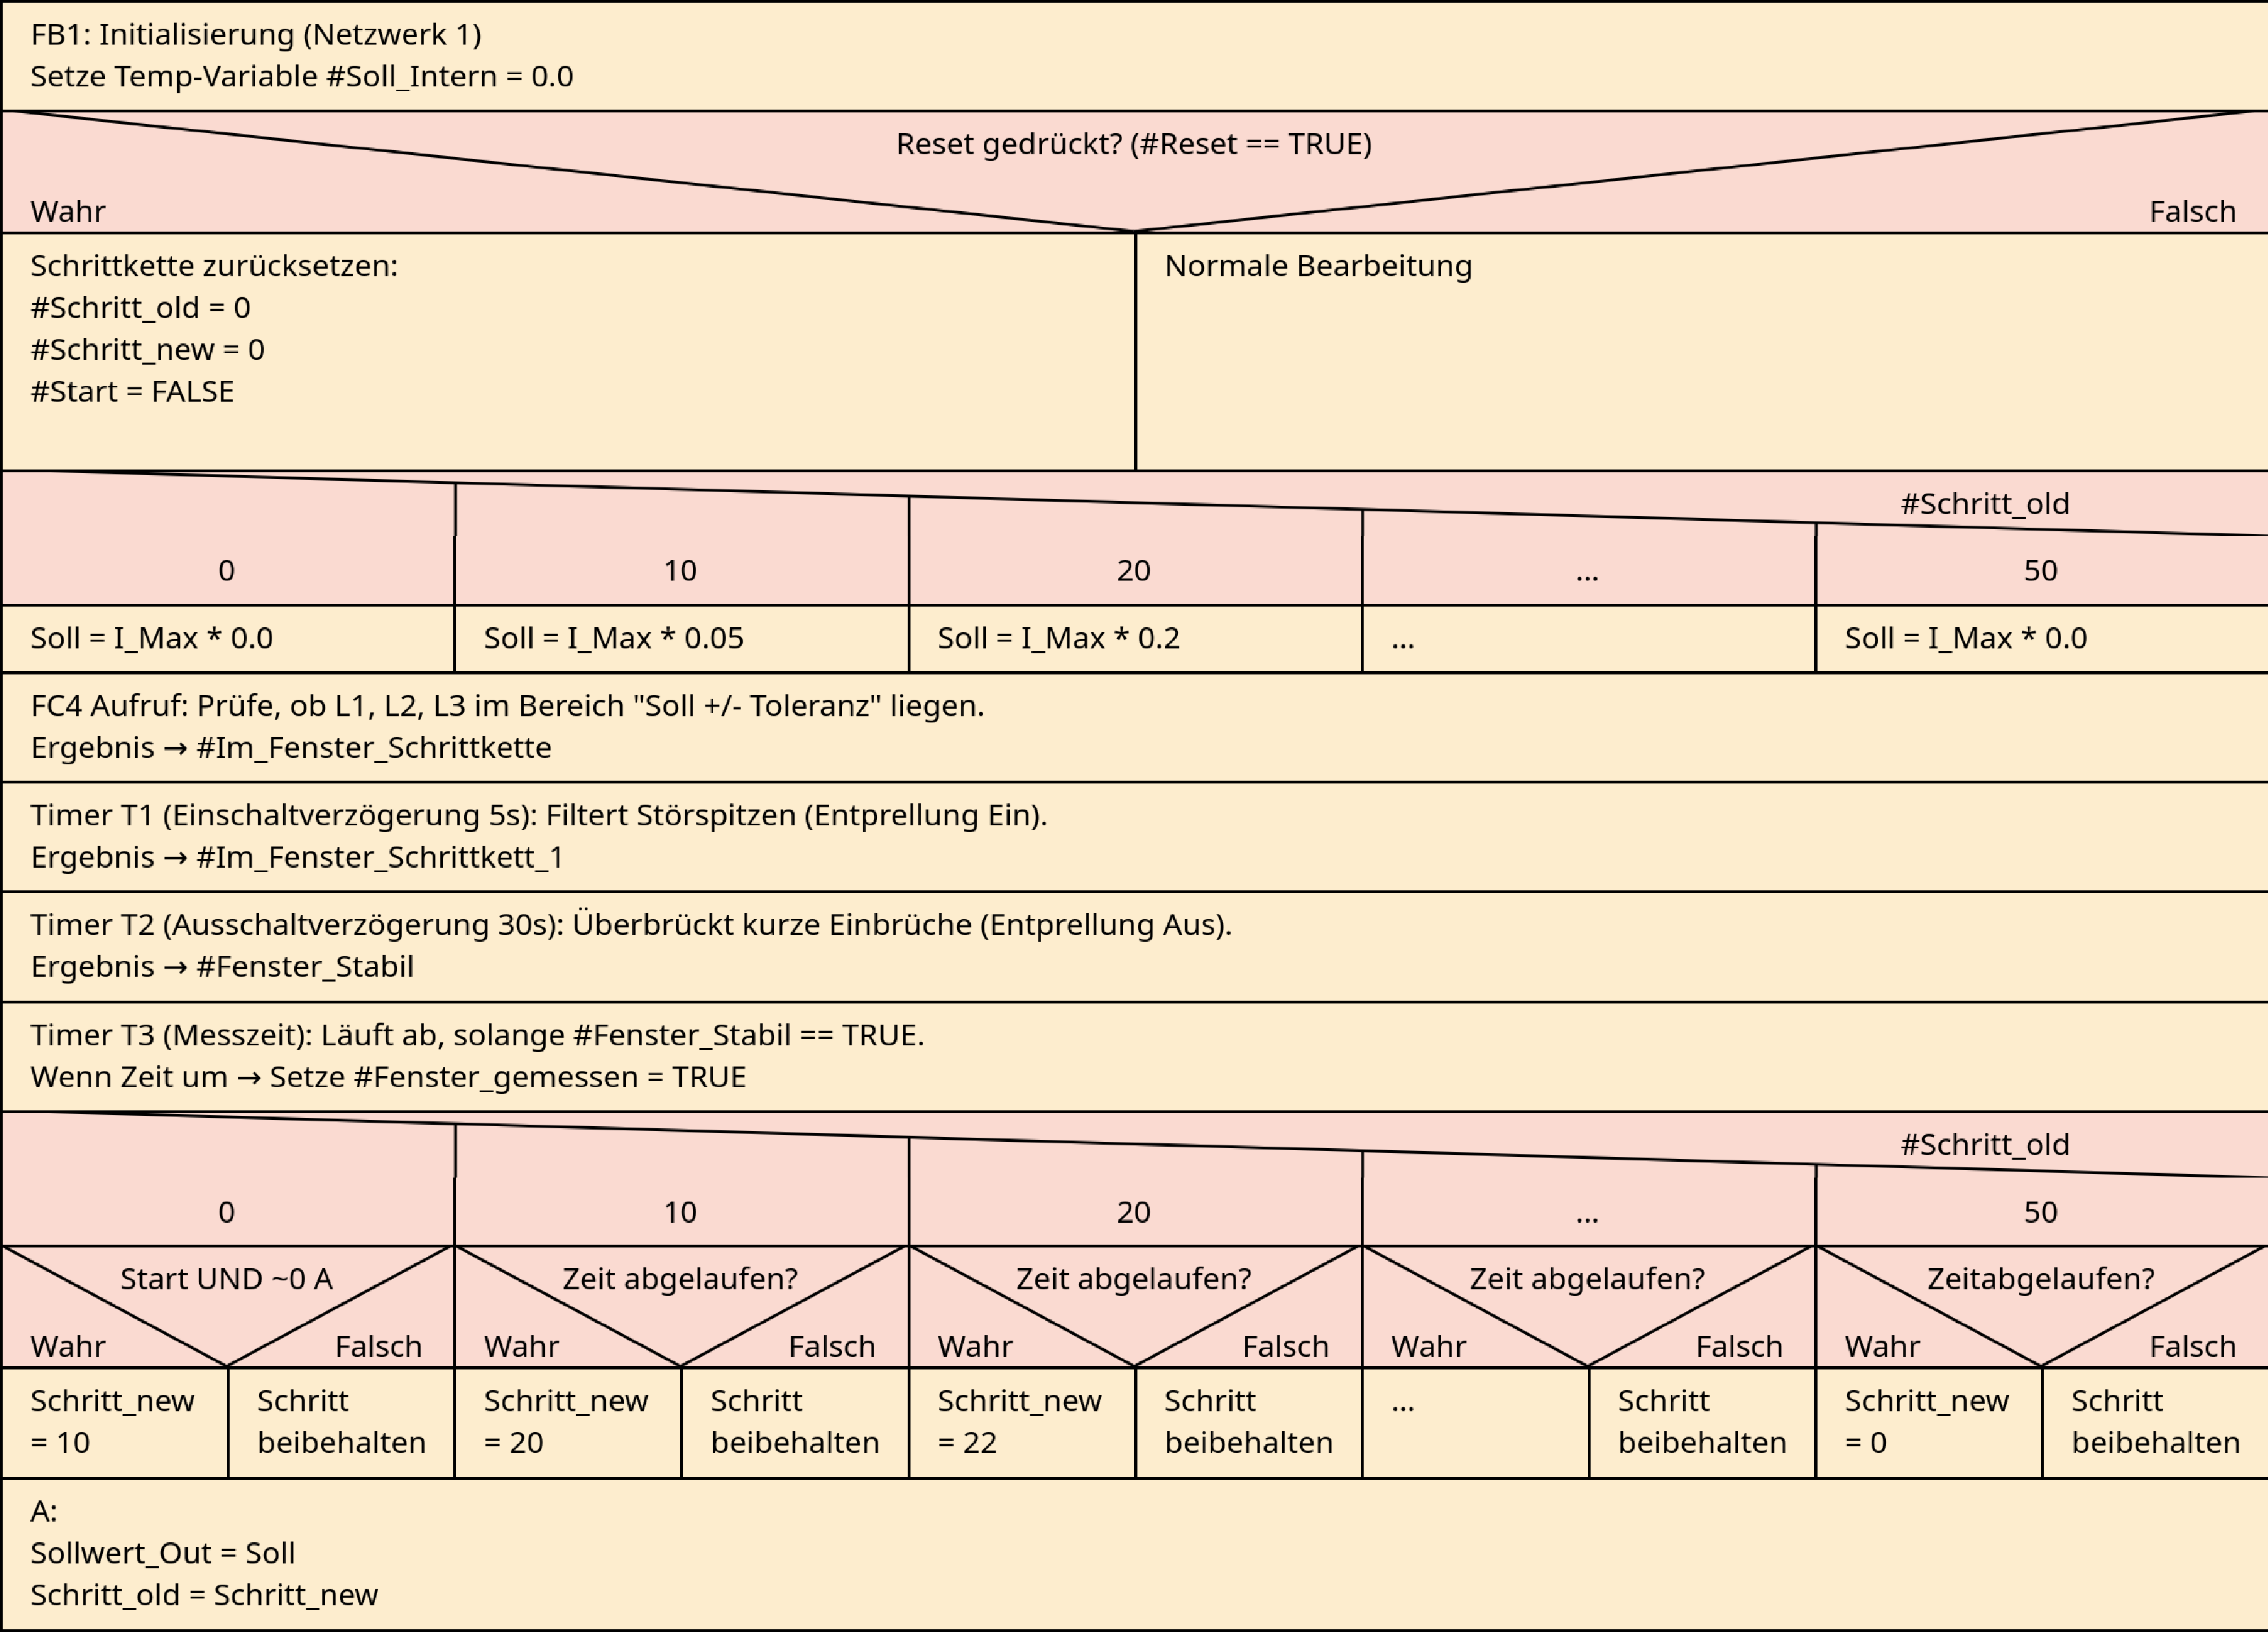
\includegraphics[width=1.0\textwidth]{03_Ressourcen/pdf/step7_programm/strukto_fb1.pdf}
    \caption{Struktogramm der Schrittkette zur automatisierten Kennlinienaufnahme (\gls{fb}1)}
    \label{pic:strukto_fb1}
\end{figure}

Der logische Ablauf dieser Automatisierung ist im Struktogramm des Funktionsbausteins \gls{fb}1 dargestellt.
Der Baustein übernimmt die zentrale Steuerung, wobei zu Beginn eine Initialisierung erfolgt, bei der die interne Sollwert-Variable auf Null gesetzt wird.
Im Falle eines aktiven Reset-Signals wird die gesamte Schrittkette zurückgesetzt, indem die Schrittzähler auf Null und das Startsignal auf den Zustand Falsch gesetzt werden.
Während der normalen Bearbeitung wird basierend auf dem aktuellen Schrittwert der entsprechende Sollwert für den Primärstrom vorgegeben.
So entspricht beispielsweise Schritt 10 einer Last von 5~\% und Schritt 20 einer Last von 20~\% des Maximalstroms.
Zur Überprüfung der Messwertstabilität wird die Funktion \gls{fc}4 aufgerufen, welche kontrolliert, ob die Phasenströme innerhalb eines definierten Toleranzfensters um den Sollwert liegen.
Ein Zeitglied T1 dient dabei der Entprellung beim Eintritt in das Fenster, während das Zeitglied T2 kurze Einbrüche überbrückt, um eine stabile Datenbasis sicherzustellen.
Die eigentliche Messzeit wird durch den Timer T3 gesteuert, der nach Ablauf die Messung am aktuellen Punkt als abgeschlossen markiert.
Die Weiterschaltlogik der Schrittkette wertet diesen Status aus: Im Ausgangszustand wird auf die Startbedingungen gewartet, während in den aktiven Prüfschritten der Übergang zum nächsten Pegel erst nach erfolgreichem Ablauf der Messzeit erfolgt.
Abschließend werden der ermittelte Sollwert an den Regler ausgegeben und der Schrittstatus für den nächsten Zyklus aktualisiert.



\subsubsection{Softwaregestützte Prozesskette zur Datenauswertung}
\label{sec:datenaufbereitung_analyse}

Die vom Prüfstand exportierten Rohdaten liegen im \gls{csv}-Format vor und enthalten die zeitlichen Verläufe der Ströme $I_{prim}$ (Referenz) und $I_{sek}$ (Prüfling). Angesichts des Umfangs der Untersuchung, die 31 Konfigurationen mit jeweils zwei Messgeräten und drei Phasen umfasst, ergaben sich insgesamt über 180 auszuwertende Einzelmessreihen. Eine manuelle Verarbeitung dieser Datenmenge mittels Tabellenkalkulation wäre zeitaufwendig und anfällig für Übertragungsfehler gewesen. Aus diesem Grund wurde eine spezialisierte Auswertungssoftware in Python entwickelt.

\textbf{Extraktion und Filterung der Messdaten}

Der erste Schritt der Auswertung erfolgt im Modul \textit{„Manueller Rohdaten-Export“} (siehe Abbildung \ref{pic:manual_tagger}). Da die Datenerfassung am Prüfstand mit einer Abtastrate von \SI{2}{Hz} (zwei Messwerte pro Sekunde) erfolgt, entstehen umfangreiche Zeitreihen. Die zentrale Funktion des Rohdaten-Selektors besteht darin, die aufgezeichneten Laststufen zu analysieren und die stationären Messbereiche zu isolieren. Hierbei werden die transienten Ein- und Ausschwingvorgänge aus dem Datensatz entfernt, sodass ausschließlich die stabilen Phasen in die weiterführende Genauigkeitsberechnung einfließen.

\begin{figure}[H]
    \centering
    \includegraphics[width=1.0\textwidth]{03_Ressourcen/pdf/datenverarbeitung/rohdaten_export.png}
    \caption{Benutzeroberfläche des manuellen Rohdaten-Exports zur Selektion stabiler Messbereiche}
    \label{pic:manual_tagger}
\end{figure}

Für die Berechnung werden pro Laststufe exakt 560 Messpunkte herangezogen, was einem Zeitfenster von 4 Minuten und 40 Sekunden entspricht. Dies gewährleistet, dass für alle Messreihen eine identische statistische Basis vorliegt. Die so selektierten Bereiche werden als sortierte Datensätze in der Datenbank für die Weiterverarbeitung gespeichert.

\textbf{Mathematische Berechnung}

Die mathematische Grundlage für die in der Software dargestellten Werte bildet die Berechnung der prozentualen Messabweichung $\varepsilon$ gemäß Abschnitt \ref{sec:messabweichung_fehlerfortpflanzung}.
Für die automatisierte Auswertung werden zunächst die arithmetischen Mittelwerte der Ströme über das stabile Zeitfenster (560 Messpunkte) gebildet und anschließend verrechnet:

\begin{equation}
    \label{eq:messabweichung_allg}
    \varepsilon = \frac{\bar{I}_{ist} - \bar{I}_{ref}}{\bar{I}_{ref}} \cdot 100\,\%
\end{equation}

Hierbei beschreibt $\bar{I}_{ist}$ den arithmetischen Mittelwert der gemessenen Stromstärke des Prüflings und $\bar{I}_{ref}$ den Mittelwert des Referenzmessgerätes im gleichen Zeitraum.
Ergänzend hierzu berechnet die Software die Standardabweichung $\sigma$ auf Basis der Einzelmesswerte $x_i$, um die Signalstabilität (Rauschen) innerhalb des Plateaus zu quantifizieren:

\begin{equation}
    \label{eq:standardabweichung}
    \sigma = \sqrt{\frac{1}{N-1} \sum_{i=1}^{N} (x_i - \bar{x})^2}
\end{equation}

Diese statistische Kenngröße dient als Indikator für die Güte der Regelung und die Ruhe des Messsignals.

\textbf{Analyse und Visualisierung}

Nachdem die Berechnungen abgeschlossen und in der Datenbank gespeichert sind, stehen die Ergebnisse in zwei spezialisierten Analyse-Tabs zur Verfügung.

Der Reiter \textbf{„Gesamtgenauigkeit“} ermöglicht den detaillierten technischen Vergleich. Hier wird die prozentuale Messabweichung über dem Primärstrom aufgetragen. Die Darstellung ist frei konfigurierbar, sodass verschiedene Wandlertechnologien oder Messreihen direkt übereinandergelegt und visuell mit den normativen Fehlergrenzen (z.\,B. Klasse 1) verglichen werden können.

Für eine bewertende Übersicht dient der Reiter \textbf{„Ökonomische Analyse“}. Um die Komplexität der Kennlinien für einen direkten Vergleich zu reduzieren, fasst die Software die Messabweichungen in drei signifikante Betriebsbereiche zusammen:

\begin{itemize}
    \item \textbf{Niederstrombereich:} Erfasst das Anlaufverhalten und die Genauigkeit bei geringer Last (z.\,B. 5\,\% und 20\,\% $I_n$).
    \item \textbf{Nennstrombereich:} Bildet den Hauptarbeitsbereich um den Nennstrom ab (z.\,B. 50\,\% bis 100\,\% $I_n$).
    \item \textbf{Überstrombereich:} Visualisiert das Verhalten bei Überlast (z.\,B. 120\,\% $I_n$).
\end{itemize}

Um für diese Bereiche einen einzelnen, vergleichbaren Gütefaktor zu erhalten, werden die prozentualen Messabweichungen $\varepsilon$ der zugehörigen Lastpunkte aggregiert. Hierfür wird der arithmetische Mittelwert der Absolutbeträge gebildet. Dies verhindert, dass sich positive und negative Abweichungen gegenseitig kompensieren (z.\,B. $+0,5\,\%$ und $-0,5\,\%$), und stellt die durchschnittliche Betragsabweichung des Wandlers in diesem Arbeitsbereich dar:

\begin{equation}
    \label{eq:fehler_bereich}
    \bar{\varepsilon}_{Bereich} = \frac{1}{k} \sum_{j=1}^{k} |\varepsilon_j|
\end{equation}

Dabei ist $k$ die Anzahl der angefahrenen Lastpunkte innerhalb des definierten Bereichs und $|\varepsilon_j|$ der Betrag der Messabweichung am jeweiligen Prüfpunkt.

In dieser Ansicht werden zudem konstruktive und wirtschaftliche Parameter, wie das Gehäusevolumen und der Preis der Wandler, den aggregierten Genauigkeitswerten gegenübergestellt. Dies ermöglicht eine multidimensionale Bewertung der Prüflinge hinsichtlich ihres Preis-Leistungs-Verhältnisses.


Durch diese Auswahl an Visualisierungen kann der Anwender je nach Fragestellung – ob rein technisch, wirtschaftlich oder konstruktiv – die geeignete Darstellungsform wählen, um eine fundierte Auswahlentscheidung für den optimalen Stromwandler zu treffen.


\subsubsection{Auswertung der neuen Messstrecke}
\label{sec:auswertung_messstrecke}

Die Validierung der optimierten Messstrecke belegt eine Steigerung der Messgüte im Vergleich zu den ursprünglichen Komponenten. In Abbildung \ref{dia:messstrecke_neu} ist der Fehlerverlauf des neu installierten Energiemessgerätes PAC 4220 (magenta) im direkten Vergleich zum Messumformer K-3 (grün) und den Rogowskispulen (blau) dargestellt. Der Kurvenverlauf verdeutlicht, dass das PAC 4220 über nahezu den gesamten Lastbereich innerhalb des normativen Toleranzbandes der Genauigkeitsklasse 0,2 verbleibt. Ab einer Last von 20\,\% des Nennstroms stabilisiert sich die Messabweichung nahe der Nulllinie.

\begin{diagram}[H]
    \centering
    \includegraphics[width=1.0\textwidth]{03_Ressourcen/diagramme/dia_messstrecke_neu/dia_messstrecke_neu-Zusammenfassung_MultiCurrent.pdf}
    \caption{Vergleichende Analyse der Messabweichung (oben) und Standardabweichung (unten) unter Einsatz des PAC 4220}
    \label{dia:messstrecke_neu}
\end{diagram}

Eine Abweichung außerhalb der Normgrenzen ist lediglich im Bereich geringer Ströme (5\,\%) erkennbar. Wie in Abschnitt \ref{sec:fehleranalyse} erläutert, resultiert dieser Effekt aus dem begrenzten Stellbereich des Säulenstelltransformators, der bei minimaler Auslenkung keine stabile Stromvorgabe ermöglicht. Durch die hohe Auflösung des PAC 4220 lässt sich diese physikalische Grenze des Prüfstandes messtechnisch präzise erfassen.

Die im unteren Teil der Abbildung \ref{dia:messstrecke_neu} visualisierte Standardabweichung dient als Maß für die Präzision und Reproduzierbarkeit der Messsysteme. Hierbei weisen das PAC 4220 und der Messumformer K-3 ein ähnliches Verhalten mit einer geringen Streuung auf. Ab einer Last von 50\,\% sinkt die Standardabweichung für beide Geräte auf ein Niveau von unter 0,5\,\%. Im Gegensatz dazu zeigen die Rogowskispulen über den gesamten Messbereich eine höhere Streuung. Obwohl die K-3-Umformer eine vergleichbare Präzision wie das PAC-Messgerät erzielen, verbleiben sie aufgrund ihrer hohen systematischen Abweichung außerhalb der geforderten Genauigkeitsklasse.

Ergänzend zur Analyse der Einzelabweichungen ermöglicht das Ökonomie-Ranking in Abbildung \ref{dia:oekonomie_ranking} eine zusammenfassende Bewertung der Messsysteme.

\begin{diagram}[H]
    \centering
    \includegraphics[width=1.0\textwidth]{03_Ressourcen/diagramme/dia_messstrecke_neu/dia_messstrecke_neu-Oekonomie_Ranking.pdf}
    \caption{Kumulierter Vergleich der Fehleranteile (Ökonomie-Ranking) der verschiedenen Messsysteme über drei Lastbereiche}
    \label{dia:oekonomie_ranking}
\end{diagram}

Hierbei werden die kumulierten Fehleranteile in den Bereichen Niederstrom (blau), Nennstrom (rot) und Überlast (gelb) gegenübergestellt. Zur quantitativen Bewertung dieser Anteile dient der in Tabelle \ref{tab:fehler_score_vergleich} ausgewiesene Fehler-Score.

\begin{table}[H]
    \centering
    \caption{Vergleichende Übersicht der Fehleranteile und des resultierenden Fehler-Scores der Messsysteme.}
    \label{tab:fehler_score_vergleich}
    \begin{tabular}{lcccc}
        \hline
        \textbf{Messsystem} & \textbf{Niederstrom [\%]} & \textbf{Nennstrom [\%]} & \textbf{Überlast [\%]} & \textbf{Fehler-Score [\%]} \\ \hline
        PAC 4220            & 13,10                     & 2,00                    & 0,96                   & 16,06                      \\
        K-3                 & 100,00                    & 41,19                   & 15,36                  & 156,55                     \\
        Rogowski-Spulen     & 84,50                     & 100,00                  & 100,00                 & 284,50                     \\ \hline
    \end{tabular}
\end{table}

Dieser Score berechnet sich aus der Summe der Abweichungen über alle Lastbereiche, wobei ein niedriger Wert eine höhere Gesamtgenauigkeit indiziert. Im direkten Vergleich erreicht das PAC 4220 einen Fehler-Score von 16,06\,\%, während der Messumformer K-3 einen kumulierten Anteil von 156,55\,\% aufweist. Die Rogowski-Spulen markieren mit 284,50\,\% die größte Abweichung im Vergleich. Diese Ergebnisse bestätigen, dass erst durch den Einsatz der digitalen PAC-Messgeräte eine valide Datenbasis geschaffen wurde, die sowohl eine geringe Streuung als auch eine normgerechte Genauigkeit für die Charakterisierung der Stromwandler vereint.

\subsubsection{Auswahl und Spezifikation der Messstromwandler}
\label{sec:auswahl_wandler}

Für die experimentellen Untersuchungen werden Stromwandler der Hersteller MBS, Celsa und Redur eingesetzt.
Die Auswahl deckt ein Spektrum von marktüblichen Standardwandlern bis hin zu spezialisierten Modellen mit integriertem Fremdfeldschutz ab.
Ziel dieser Zusammenstellung ist es, eine belastbare Datenbasis für die Analyse der Beeinflussungseffekte unter verschiedenen technologischen Voraussetzungen zu schaffen.
Tabelle \ref{tab:wandler_spezifikationen_erweitert} fasst die technischen Kenndaten der Prüflinge zusammen. Neben dem Nennstrom $I_n$ und der Bemessungsleistung $S_n$ ist das Gehäusevolumen aufgeführt.
Dieses dient als Vergleichsgröße für die Wirtschaftlichkeitsbetrachtung und errechnet sich aus dem Produkt der maximalen äußeren Gehäuseabmessungen (Höhe $\times$ Breite $\times$ Tiefe).
Es ist anzumerken, dass es sich hierbei um eine Vereinfachung handelt, die den Wandler auf seinen quaderförmigen Hüllkörper reduziert.
Spezifische Geometrien, wie etwa Verjüngungen oder Abrundungen am Gehäuse, werden in dieser Berechnung vernachlässigt, sodass das tatsächliche Materialvolumen geringer ausfallen kann.
Für die konstruktive Bewertung in Schaltanlagen ist diese Betrachtungsweise jedoch maßgeblich, da für die Montageplanung der maximale Platzbedarf (Bauraum) reserviert werden muss, den der Wandler im Anschlussraum effektiv beansprucht.
\begin{table}[H]
    \centering
    \caption{Erweiterte Spezifikationen und wirtschaftliche Kennwerte der Prüflinge}
    \label{tab:wandler_spezifikationen_erweitert}
    \begin{tabular}{@{}lll
            S[table-format=4.0]
            S[table-format=2.1]
            S[table-format=4.0]
            S@{}}
        \toprule
        \textbf{Hersteller}
                                                     & 
        \textbf{Typ}                                 & 
        \textbf{Technologie}                         & 
        {\textbf{$I_n$ [\si{\ampere}]}}
                                                     & 
        {\textbf{$S_n$ [\si{\volt\ampere}]}}         & 
        {\textbf{Volumen [\si{\centi\meter\cubed}]}} & 
        \textbf{Preis [\euro]}
        \\
        \midrule
        Celsa                                        & ALO 10030
                                                     & Standard      & 2000        & 2,5  & 634,3 & 45,50           \\
        Celsa                                        & ALO 8030 K    & Kompensiert & 2000 & 10,0  & 710,2  & 95,95  \\
        Celsa
                                                     & ALO 10030     & Standard    & 2500 & 2,5   & 634,3  & 45,50  \\
        Celsa
                                                     & ALO 10050 K   & Kompensiert & 2500 & 5,0   & 1027,0 & 104,20 \\
        Celsa                                        & ALO 12070     & Standard    & 3000 & 15,0  & 1520,0 & 71,51  \\
        Celsa
                                                     & ALO 12070 K   & Kompensiert & 3000 & 15,0  & 1520,0 & 346,06 \\
        Celsa
                                                     & ALO 12070     & Standard    & 4000 & 15,0  & 1520,0 & 71,51  \\
        Celsa                                        & ALO 12070 K   & Kompensiert & 4000 & 15,0  & 1520,0 & 401,91 \\
        Celsa
                                                     & ALO 20060     & Standard    & 5000 & 40,0  & 1989,0 & 124,76 \\
        Celsa
                                                     & ALO E 16050 K & Kompensiert & 5000 & 40,0  & 1903,0 & 414,56 \\
        \addlinespace
        MBS                                          & ASK 101.4     & Standard    & 2000 & 10,0  & 733,2  & 141,90 \\
        
        MBS                                          & ASK 129.10    & Standard    & 5000 & 15,0  & 6175,0 & 303,10 \\
        \addlinespace
        Redur
                                                     & 13A1030.3ffp  & FFP         & 2000 & 10,0  & 778,7  & ??
        \\
        Redur                                        & 20A1456.5vffp & VFFP        & 5000 & 15,0  & 1600,0 & ??
        \\
        \bottomrule
    \end{tabular}
\end{table}



Die eingesetzten Wandler lassen sich technologisch in drei Kategorien unterteilen.
Als Basis dienen Standardwandler, die einen klassischen Aufbau ohne zusätzliche konstruktive Schutzmaßnahmen gegen externe Felder aufweisen (siehe Abschnitt \ref{sec:aufbau_wandler}).
Eine weiterführende Bauform stellen die kompensierten Wandler dar. Diese Modelle verfügen über eine modifizierte Wicklungsanordnung, die gezielt zur Reduktion von Messabweichungen bei asymmetrischer Primärleiterlage eingesetzt wird (siehe Abschnitt \ref{sec:kompensationswicklungen}).
Die dritte Gruppe bilden die spezialisierten \gls{ffp}- und VFFP-Wandler der Firma Redur, die die Technologie der Fremdfeldprotektoren nutzen.
Die Bezeichnung \gls{ffp} steht für \textit{Fremdfeldprotektoren}. Diese Technologie wurde entwickelt, um den Eintritt magnetischer Fremdfelder in den Wandlerkern zu verringern.
Der Hersteller unterteilt die Protektoren in Klassen wie FFP1, FFP5 und FFP10, welche den Grad der Schirmwirkung definieren.
Technisch wird dies durch die Integration eines Werkstoffs mit hoher magnetischer Permeabilität am oder im Gehäuse des Wandlers realisiert.
Diese Schirmung fungiert als magnetischer Shunt, der die Feldlinien benachbarter Leiter um den Messkern herumleitet.
Infolgedessen bleibt die magnetische Induktion im Kernmaterial weitgehend unbeeinflusst von äußeren Feldern \cite{Redur2021Fremdfeld}.
Um die Vergleichbarkeit der Messergebnisse zu gewährleisten, entsprechen alle ausgewählten Wandler der Genauigkeitsklasse 1,0.
Die in der Tabelle aufgeführten Nennbürden sind so gewählt, dass sie die Anforderungen für die in Abschnitt \ref{sec:integration_programmierung} beschriebene thermische Dauerbelastung erfüllen.

\subsubsection{Geometrische Anordnung der Primärleiter}
\label{sec:layout_geometrie}

In Niederspannungsschaltanlagen werden Kupferschienen vorwiegend parallel angeordnet. Diese Bauweise zeichnet sich durch Platzersparnis und eine geringe Montagekomplexität aus. Die Führung der Schienen wird konstruktiv maßgeblich durch die Anschlüsse des Leistungsschalters bestimmt. Daher sind Variationen der Geometrie im realen Anlagenbau nur eingeschränkt möglich. Die Messstromwandler werden üblicherweise dem Hauptschalter nachgelagert im Anschlussraum installiert. Aufgrund des begrenzten Bauraums stellt die Realisierung abweichender Leiteranordnungen wie etwa einer Dreieckskonfiguration zur Reduktion von Fremdfeldern eine konstruktive Herausforderung dar.

\begin{figure}[H]
    \centering
    \includegraphics[width=1.0\textwidth]{03_Ressourcen/Bilder/kupferschinen_gesamtaufbau.pdf}
    \caption{Technische Zeichnung des Kupferschienensystems in paralleler und dreiecksförmiger Anordnung}
    \label{pic:kupferschienen_layout}
\end{figure}


Abbildung \ref{pic:kupferschienen_layout} zeigt die konstruktive Umsetzung der untersuchten Geometrien. In der Frontalansicht ist die horizontale Führung der drei Außenleiter L1, L2 und L3 zu sehen. Die Abgangsschienen haben dabei unterschiedliche Phasenmittenabstände. Im linken Bereich (blaue Schine) beträgt der Abstand \SI{130}{mm} und im rechten Teil der Anlage (rote Schine) sind es \SI{210}{mm}. Die Seitenansicht zeigt die Umsetzung der Dreiecksanordnung. Hier ist erkennbar, dass die Schienen (grün) zur Kontaktierung der Anschlussebene zweifach gekröpft sind. Der vertikale Versatz von \SI{140}{mm} ermöglicht die räumliche Staffelung der Leiter für die Dreieckskonfiguration.


Um den Einfluss der Leitergeometrie experimentell zu untersuchen, wurde das Kupferschienensystem des Hochstromprüfstandes auf Basis dieser Zeichnung flexibel gestaltet. Dies ermöglicht den direkten Vergleich zwischen der konventionellen Parallelanordnung und einer optimierten Dreiecksanordnung bei identischen elektrischen Parametern.



Die im Versuchsaufbau gewählten Dimensionen orientieren sich an realen Industriestandards. Tabelle \ref{tab:schienen_konfiguration} gibt hierzu eine Übersicht der Phasenmittenabstände für die Leistungsschalter der Reihen 3WA12 und 3WA13, welche als Grundlage für die Konstruktion dienten.

\begin{table}[H]
    \centering
    \caption{Übersicht der Schienenkonfigurationen und Phasenmittenabstände für die Leistungsschalter 3WA12 und 3WA13 gemäß Herstellervorgaben}
    \label{tab:schienen_konfiguration}
    \begin{tabular}{lccc}
        \hline
        \textbf{Modell} & \textbf{Nennstrom} & \textbf{Schienenkonfiguration} & \textbf{Phasenmittenabstand} \\
                        & \textbf{[A]}       &                                & \textbf{[mm]}                \\ \hline
        \textbf{3WA12}  & 2000               & 2x 80x10                       & 130                          \\
                        & 2500               & 2x 100x10                      & 130                          \\ \hline
        \textbf{3WA13}  & 3200               & 3x 100x10                      & 210                          \\
                        & 4000               & 4x 100x10                      & 210                          \\
                        & 5000               & 5x 120x10                      & 210                          \\ \hline
    \end{tabular}
\end{table}

\textbf{Parallelanordnung}

Als Referenz fungiert die Parallelanordnung der drei Phasenleiter L1, L2 und L3 in einer Ebene. Dieser in Abbildung \ref{pic:kupferschienen_parallel} gezeigte Aufbau bildet die realen Bedingungen in Siemens SIVACON S8 Schaltfeldern nach. Die verwendeten Abstände entsprechen dabei den in Tabelle \ref{tab:schienen_konfiguration} aufgeführten Herstellervorgaben. In dieser Konfiguration ist der Prüfling, hier beispielhaft der Messstromwandler Redur 20A1456.5vffp (\SI{5000}{A}), den maximalen magnetischen Fremdfeldern der benachbarten Leiter ausgesetzt.

\begin{figure}[H]
    \centering
    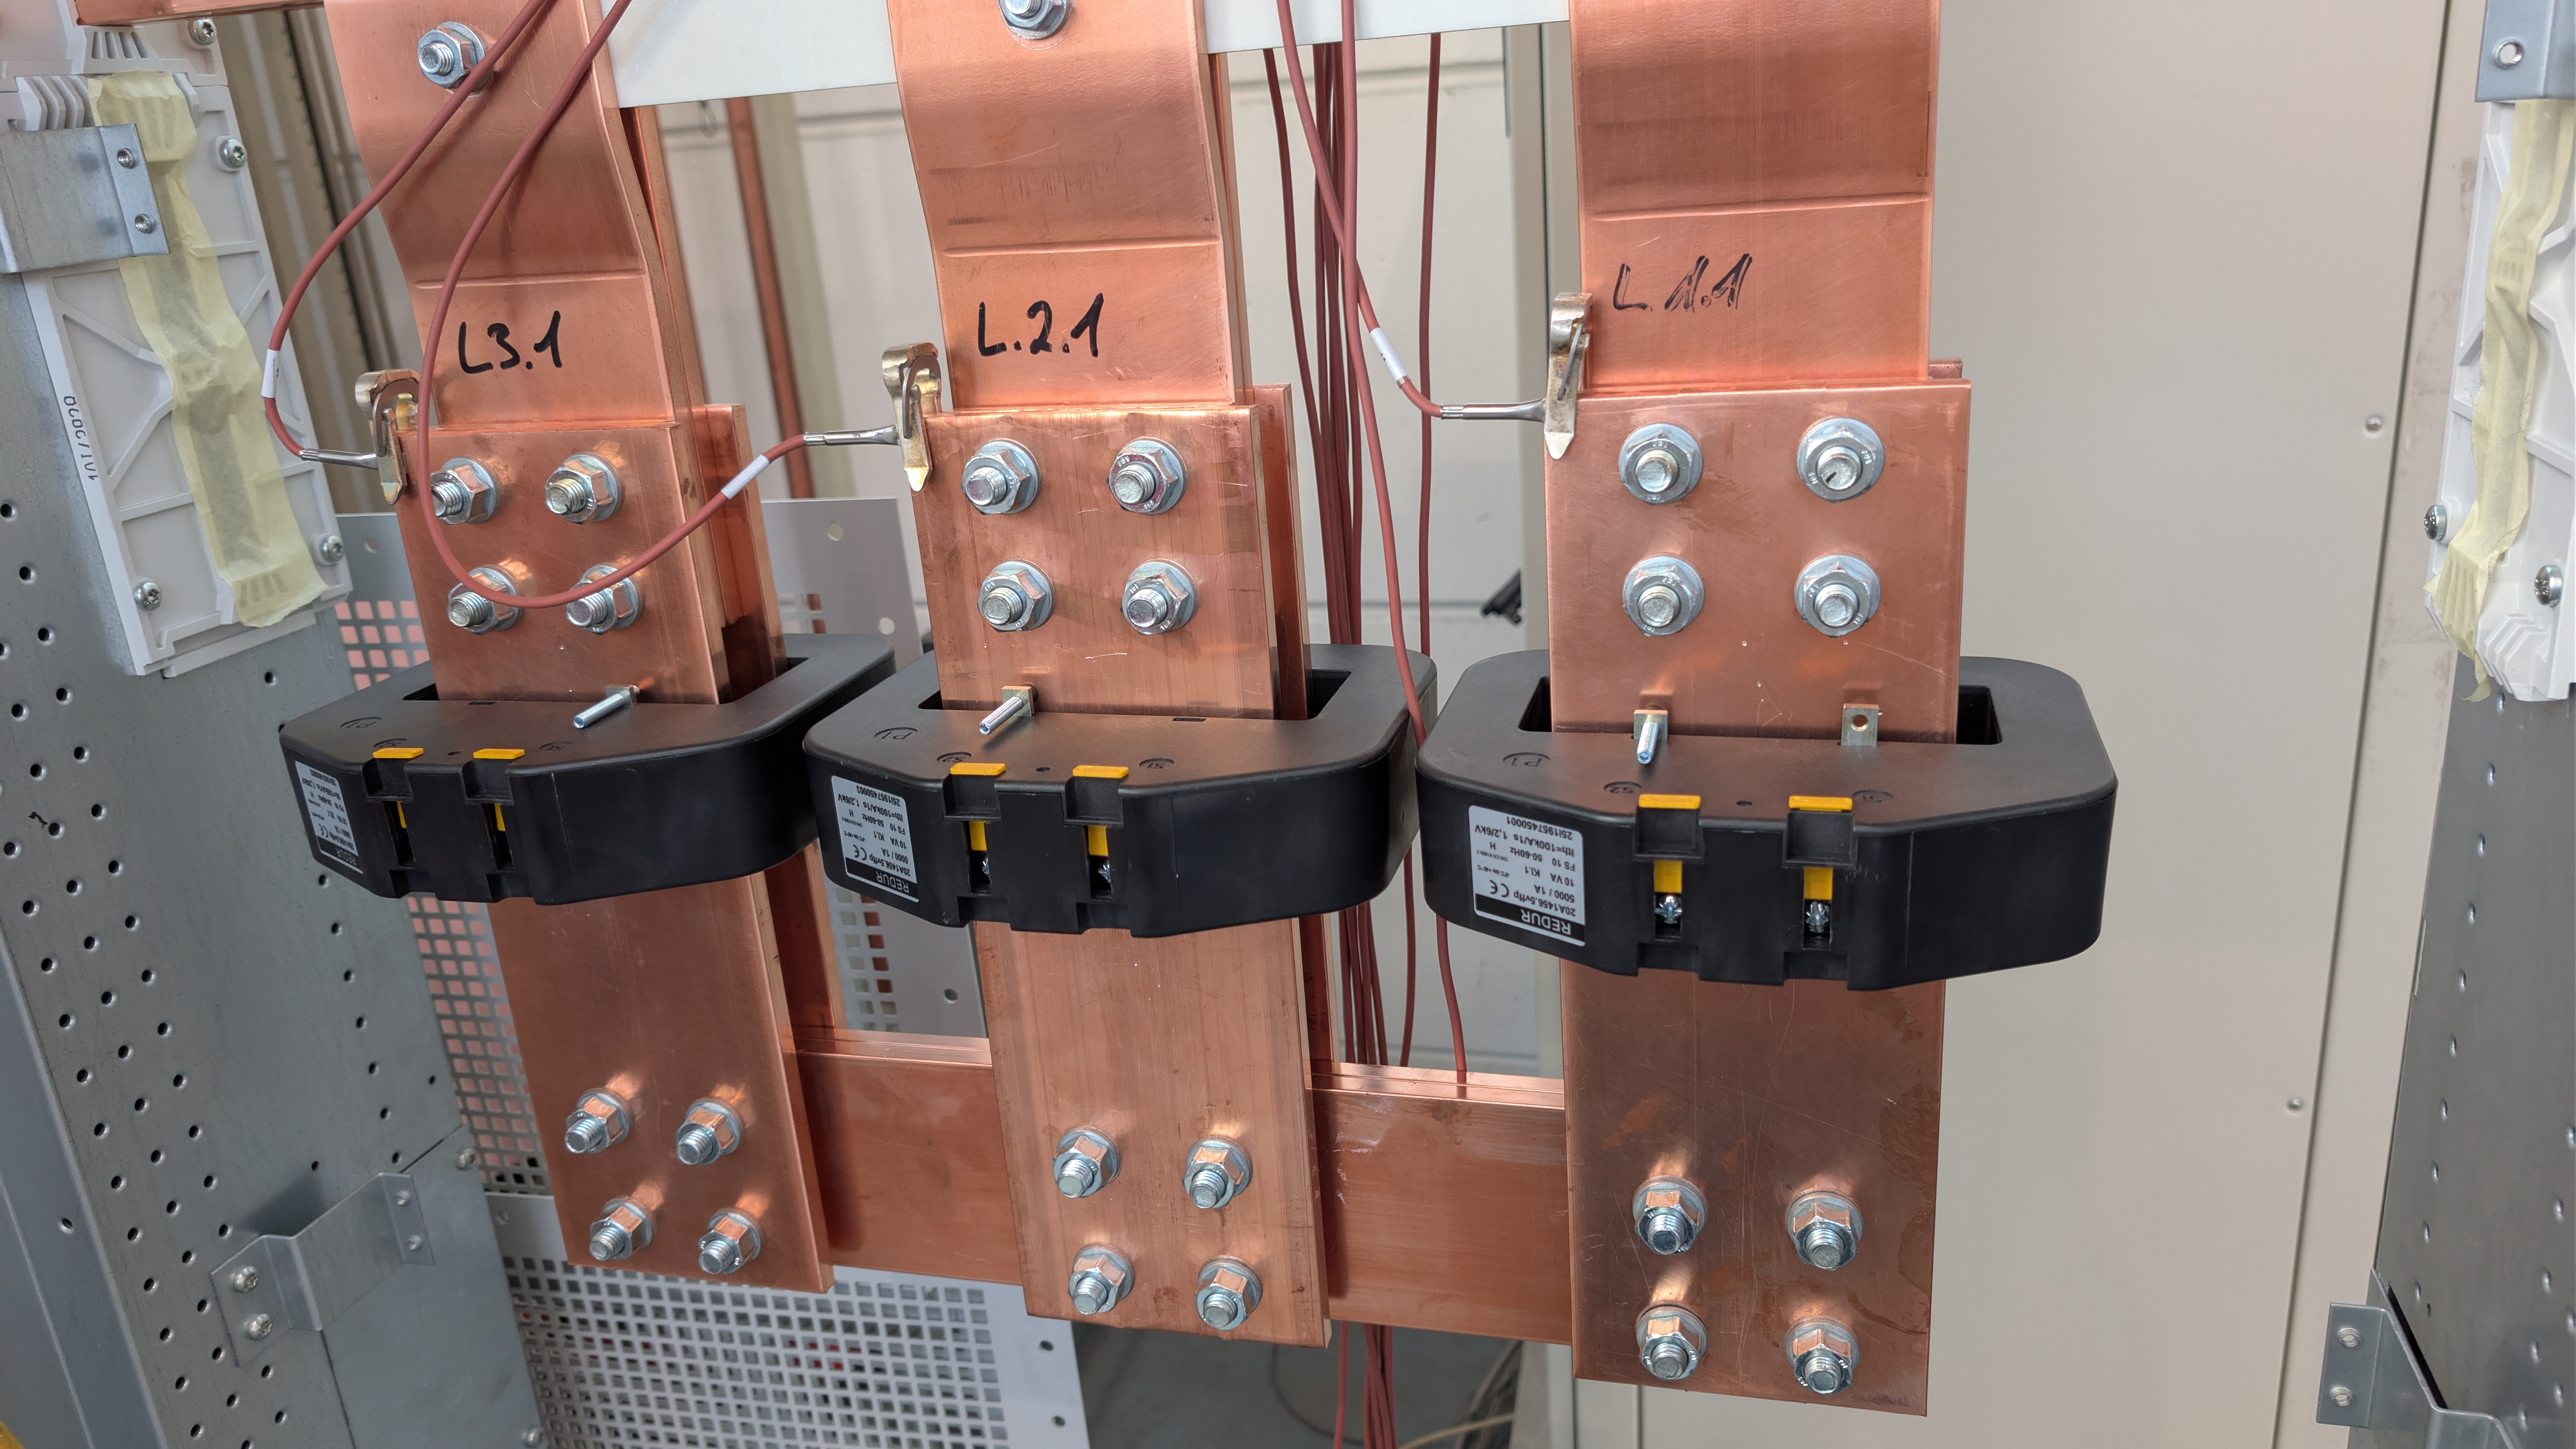
\includegraphics[width=0.8\textwidth]{03_Ressourcen/Bilder/kupferschienen_parallel.jpg}
    \caption{Versuchsaufbau in paralleler Schienenanordnung mit montiertem Messstromwandler (Typ: Redur 20A1456.5vffp)}
    \label{pic:kupferschienen_parallel}
\end{figure}

\textbf{Dreieckskonfiguration}

Für die Realisierung der Dreiecksanordnung wurde der Aufbau gemäß Abbildung \ref{pic:kupferschienen_dreieck} modifiziert. Ein speziell gefertigter Kupferadapter führt hierbei die mittlere Phase L2 geometrisch aus der Ebene der Außenleiter heraus. Der Adapter versetzt die Schiene um \SI{140,0}{mm} nach vorne. Durch diesen Versatz spannen die Mittelpunkte der drei Leiter im Querschnitt ein Dreieck auf. Ziel dieser Anordnung ist eine symmetrischere Gestaltung der magnetischen Kopplung sowie die teilweise Kompensation der vektoriellen Anteile der Fremdfelder im Bereich des Wandlerkerns. Auch in dieser Konfiguration wurde der \SI{5000}{A}-Wandler von Redur vermessen.

\begin{figure}[H]
    \centering
    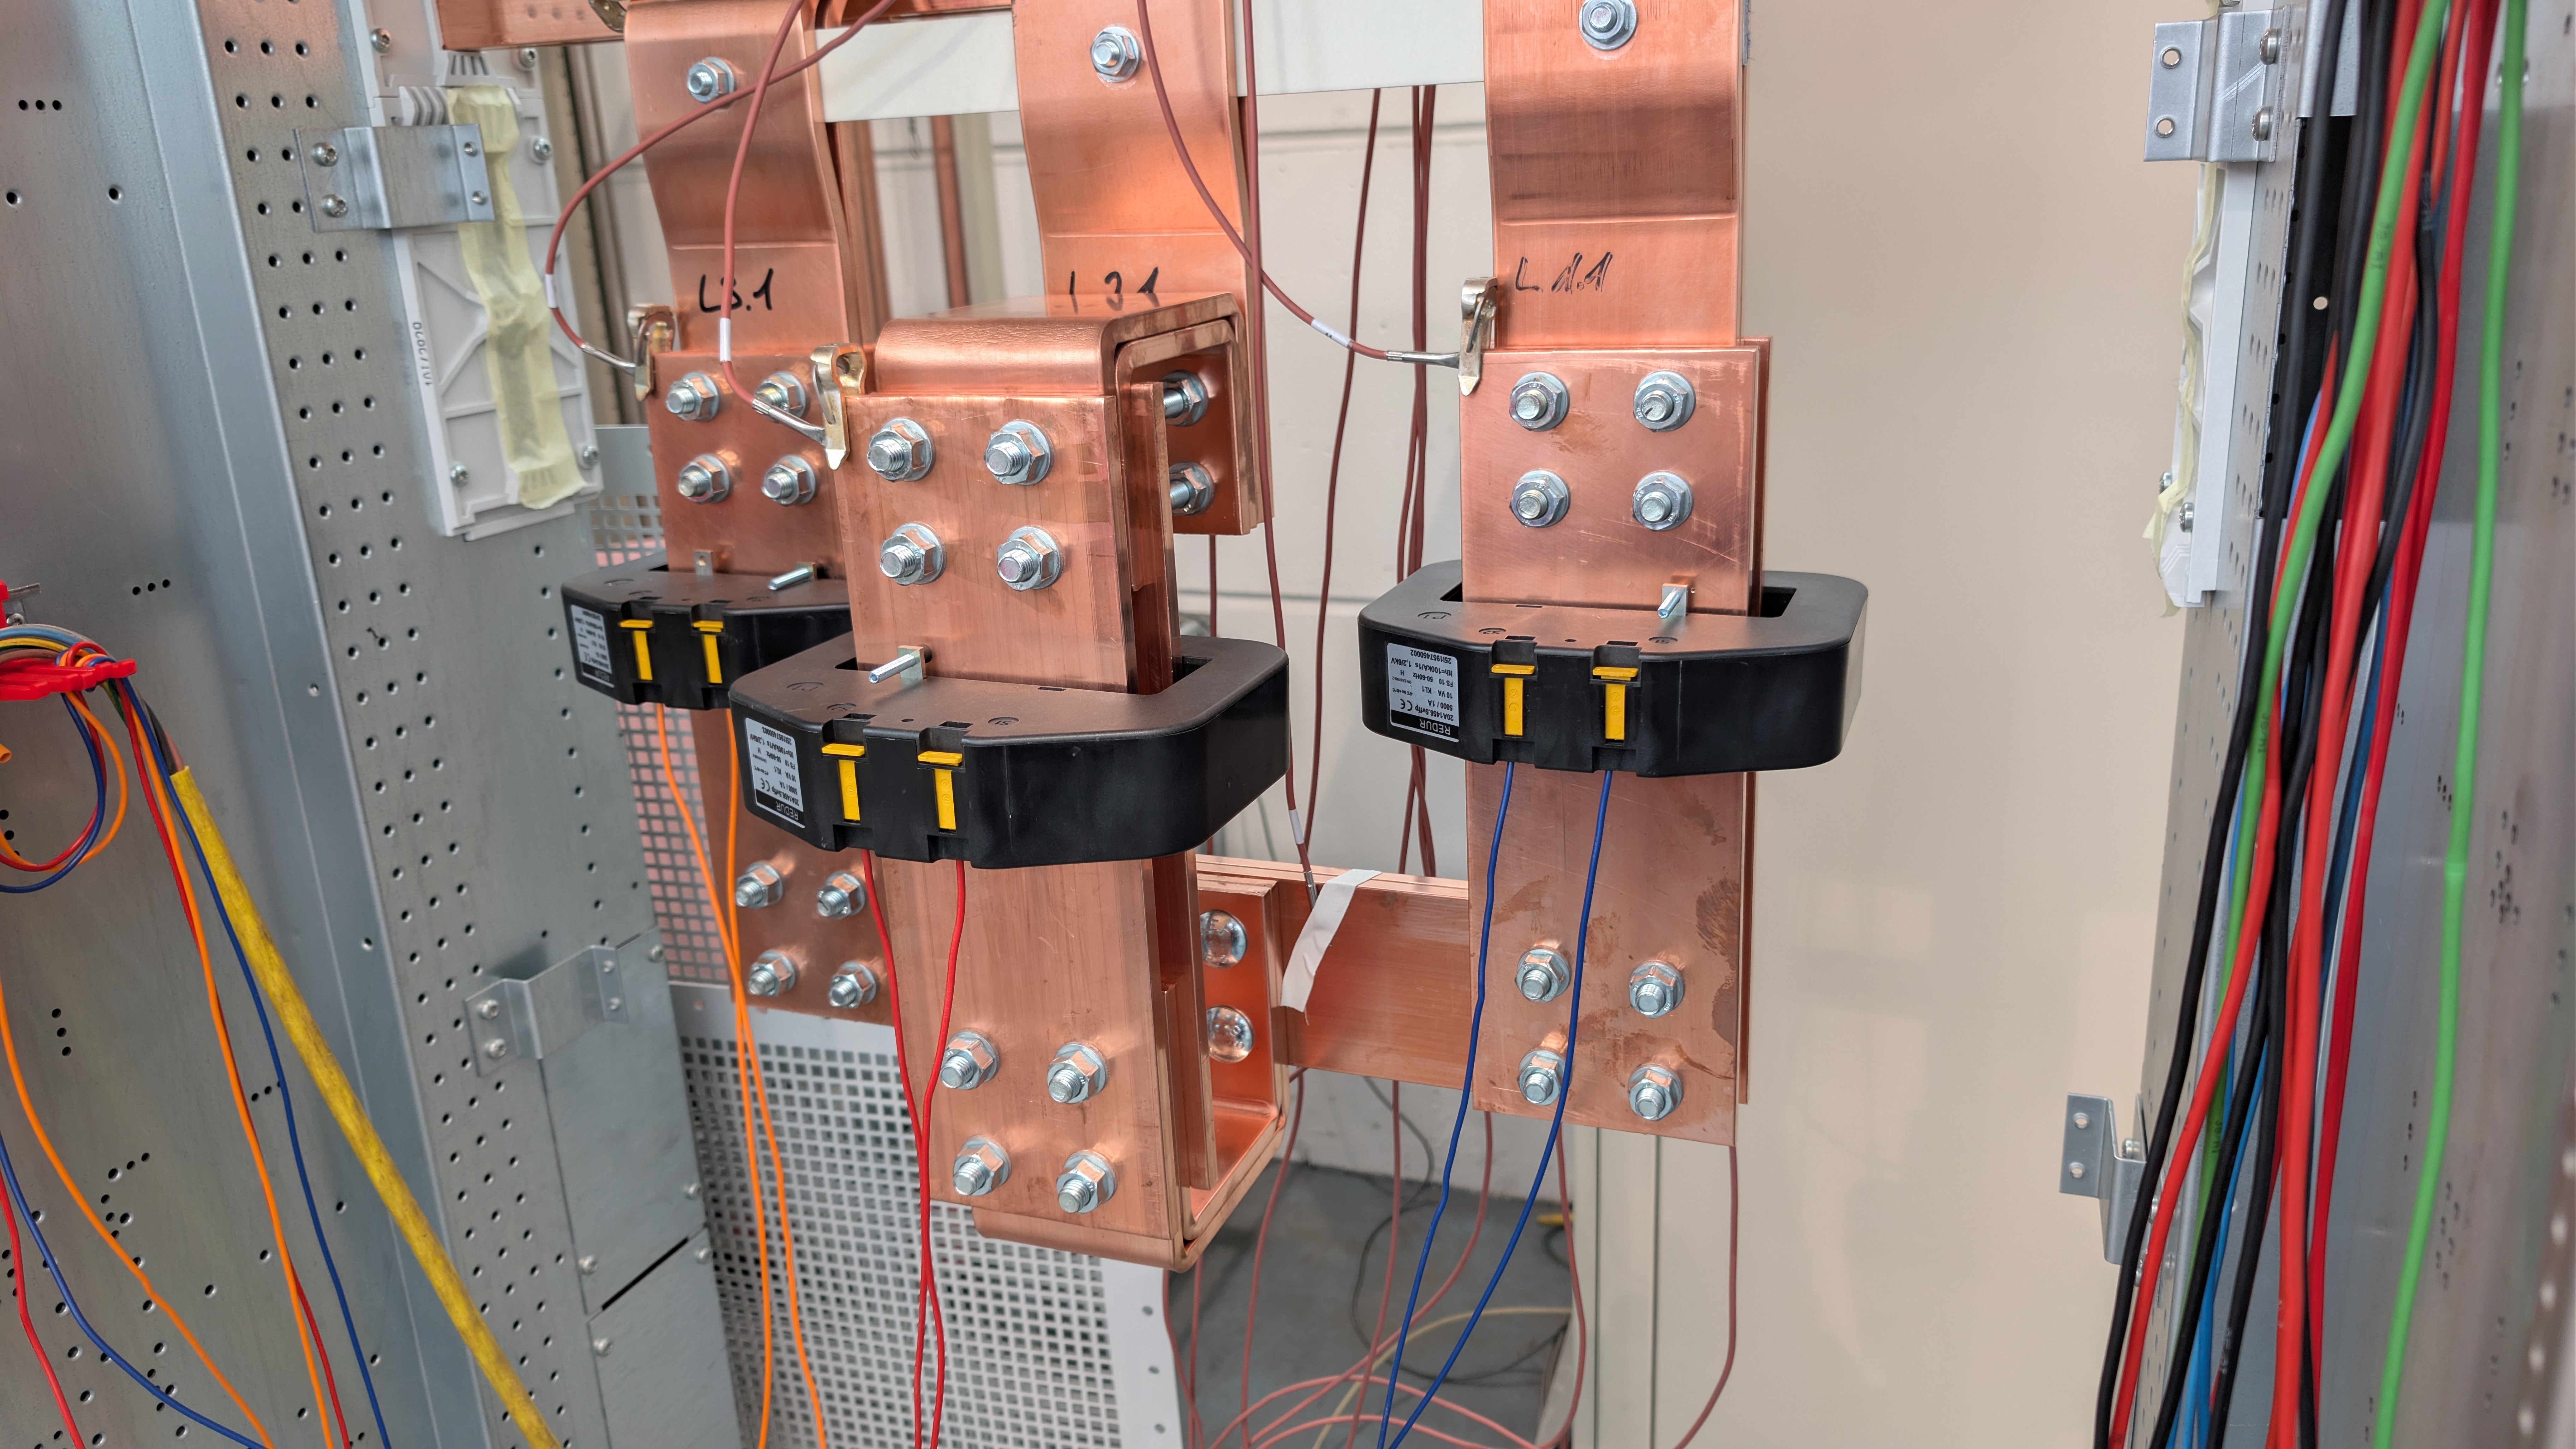
\includegraphics[width=0.8\textwidth]{03_Ressourcen/Bilder/kupferschienen_dreieck.jpg}
    \caption{Modifizierter Versuchsaufbau in Dreieckskonfiguration durch räumlichen Versatz der Phase L2 mittels Kupferadapter}
    \label{pic:kupferschienen_dreieck}
\end{figure}